\section{Structure}
\label{sec:structure}

%% Graphic of the request cycle to the build pipeline and back
\begin{figure}[b] % h-ere, t-op, b-ottom, p-age
    \centering
    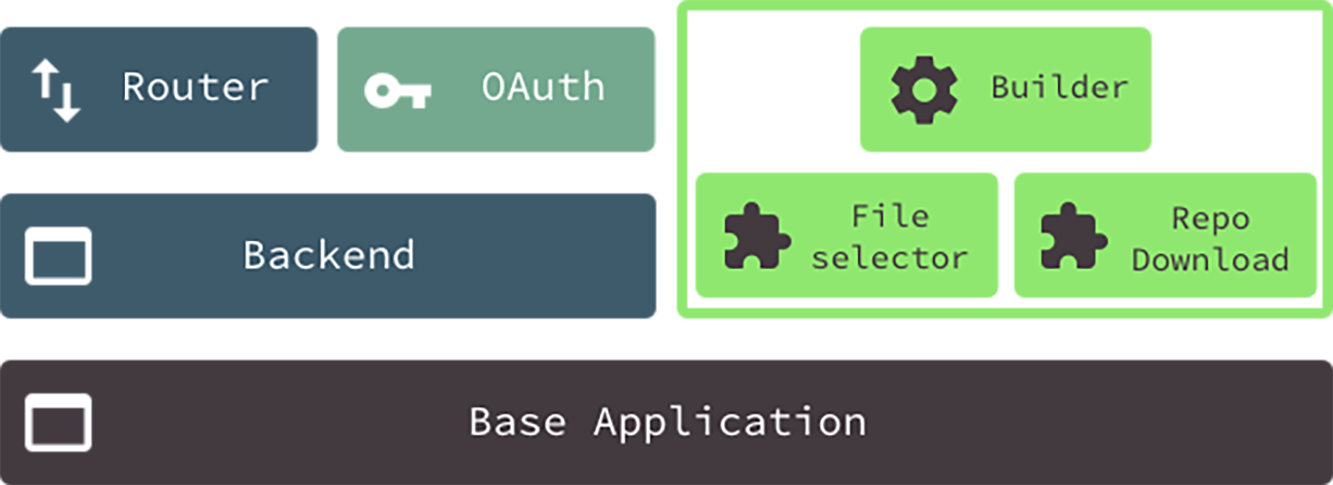
\includegraphics[width=0.9\textwidth]{application_structure.png}
    \caption{A graphic showing the base structure of the implemented application.\\ The \emph{base application} layer serves as foundation, containing necessary libraries for implementing the \emph{HTTP} specifications. The \emph{routing} and \emph{OAuth} layer are responsible for authenticated requests to the endpoints, while the \emph{builder package} is designed as a partly autonomous, loosely coupled rendering service.}
    \label{fig:application_structure}
\end{figure}
%

A basic approach of the project structure may be seen in fig. \ref{fig:application_structure}. Although this might look still very abstract, the core packages are already clearly visible, while the access neither to the GitHub API, nor to the MongoDB is yet visualized.

The graphic can be interpreted as follows:

\begin{itemize}
  \item \emph{Base application} -- Backed by Node.js, together with necessary supporting packages, such as %% MongoDB, GithubAPI
\end{itemize}
